
% This LaTeX was auto-generated from an M-file by MATLAB.
% To make changes, update the M-file and republish this document.

\documentclass{article}
\usepackage{graphicx}
\usepackage{color}

\sloppy
\definecolor{lightgray}{gray}{0.5}
\setlength{\parindent}{0pt}

\begin{document}

    
    
\subsection*{Contents}

\begin{itemize}
\setlength{\itemsep}{-1ex}
   \item 1 - Different values of P
   \item 2 - Plot for different values of P
   \item 4
   \item a - Derive P1
\end{itemize}
\begin{verbatim}
%%%%%%%%%%%%%%%%%%%%%%%%%%%%%%%%%%%%%%%%%%%%%%%%%%%%%%%%%%%%%%%%%%%%%%%%
%
%
% Zach Dischner-10/31/2012
%
% ASEN 5070-Statistical Orbit Determination
%
% Homework 8
%
%
%%%%%%%%%%%%%%%%%%%%%%%%%%%%%%%%%%%%%%%%%%%%%%%%%%%%%%%%%%%%%%%%%%%%%%%%

clc;clear all;close all; format compact;format long g;tic
\end{verbatim}


\subsection*{1 - Different values of P}

\begin{verbatim}
% Look in my function!!!
\end{verbatim}


\subsection*{2 - Plot for different values of P}

\begin{verbatim}
e           = logspace(-15,-6,1000);
P2_True     = zeros(size(e));
P2_Kalman   = P2_True;
P2_Joseph   = P2_True;
P2_Potter   = P2_True;
P2_Batch    = P2_True;

for ii = 1:length(e)
    [P2_True(ii),P2_Kalman(ii),P2_Joseph(ii),P2_Potter(ii),P2_Batch(ii)]=FindP2(e(ii),1);
end

figure
subplot(4,1,1)
loglog(e,abs(P2_True-P2_Kalman));
xlabel('\epsilon');ylabel('P2_{true} - P2_{Kalman}'); title('Kalman')
subplot(4,1,2)
loglog(e,abs(P2_True-P2_Joseph));
xlabel('\epsilon');ylabel('P2_{true} - P2_{Joseph}'); title('Joseph')
subplot(4,1,3)
loglog(e,abs(P2_True-P2_Potter));
xlabel('\epsilon');ylabel('P2_{true} - P2_{Potter}'); title('Potter')
subplot(4,1,4)
loglog(e,abs(P2_True-P2_Batch));
xlabel('\epsilon');ylabel('P2_{true} - P2_{Batch}'); title('Batch')
\end{verbatim}

\includegraphics [width=4in]{HW8main_01.eps}


\subsection*{4}



\subsection*{a - Derive P1}

\begin{verbatim}
syms err
H       = [1 2*err;1 3*err];
R       = eye(2,2);
P0bar   = (1/err^2)*eye(2,2);
P1      = inv( transpose(H)*inv(R) * H + inv(P0bar));
matlabFunction(P1,'file','Find_P1.m');
print 'The P1 Covariance matrix is:'
P1

x_batch = zeros(size(e),2);
x_kalman = x_batch;
x_joseph = x_batch;
x_potter = x_batch;

for ii = 1:length(e)
    [x_batch(ii,:),x_kalman(ii,:),x_joseph(ii,:),x_potter(ii,:),x_true(ii,:)] = FindStateP4(e(ii));
end

figure
subplot(4,2,1)
loglog(e,abs(x_true(:,1) - x_batch(:,1)));
xlabel('\epsilon');ylabel('True_1 - Batch_1'); title('batch')
subplot(4,2,3)
loglog(e,abs(x_true(:,1) - x_kalman(:,1)));
xlabel('\epsilon');ylabel('True_1 - Kalman_1'); title('Kalman')
subplot(4,2,5)
loglog(e,abs(x_true(:,1) - x_potter(:,1)));
xlabel('\epsilon');ylabel('True_1 - Potter_1'); title('Potter')
subplot(4,2,7)
loglog(e,abs(x_true(:,1) - x_joseph(:,1)));
xlabel('\epsilon');ylabel('True_1 - Joseph_1'); title('Joseph')

subplot(4,2,2)
loglog(e,abs(x_true(:,2) - x_batch(:,2)));
xlabel('\epsilon');ylabel('True_2 - Batch_2'); title('batch')
subplot(4,2,4)
loglog(e,abs(x_true(:,2) - x_kalman(:,2)));
xlabel('\epsilon');ylabel('True_2 - Kalman_2'); title('Kalman')
subplot(4,2,6)
loglog(e,abs(x_true(:,2) - x_potter(:,2)));
xlabel('\epsilon');ylabel('True_2 - Potter_2'); title('Potter')
subplot(4,2,8)
loglog(e,abs(x_true(:,2) - x_joseph(:,2)));
xlabel('\epsilon');ylabel('True_2 - Joseph_2'); title('Joseph')

figure_awesome('save')

syms e
R       = eye(2,2);
H       = [1 2*e;1 3*e];
P0bar   = [1/e^2 0;0 1/e^2];
A       = inv(P0bar) + transpose(H)*R*H;
Ptrue   = inv(A);
\end{verbatim}

        \color{lightgray} \begin{verbatim}P1 =
[     14/(14*err^2 + 3),            -5/(14*err^3 + 3*err)]
[ -5/(14*err^3 + 3*err), (err^2 + 2)/(14*err^4 + 3*err^2)]

\end{verbatim} \color{black}
    
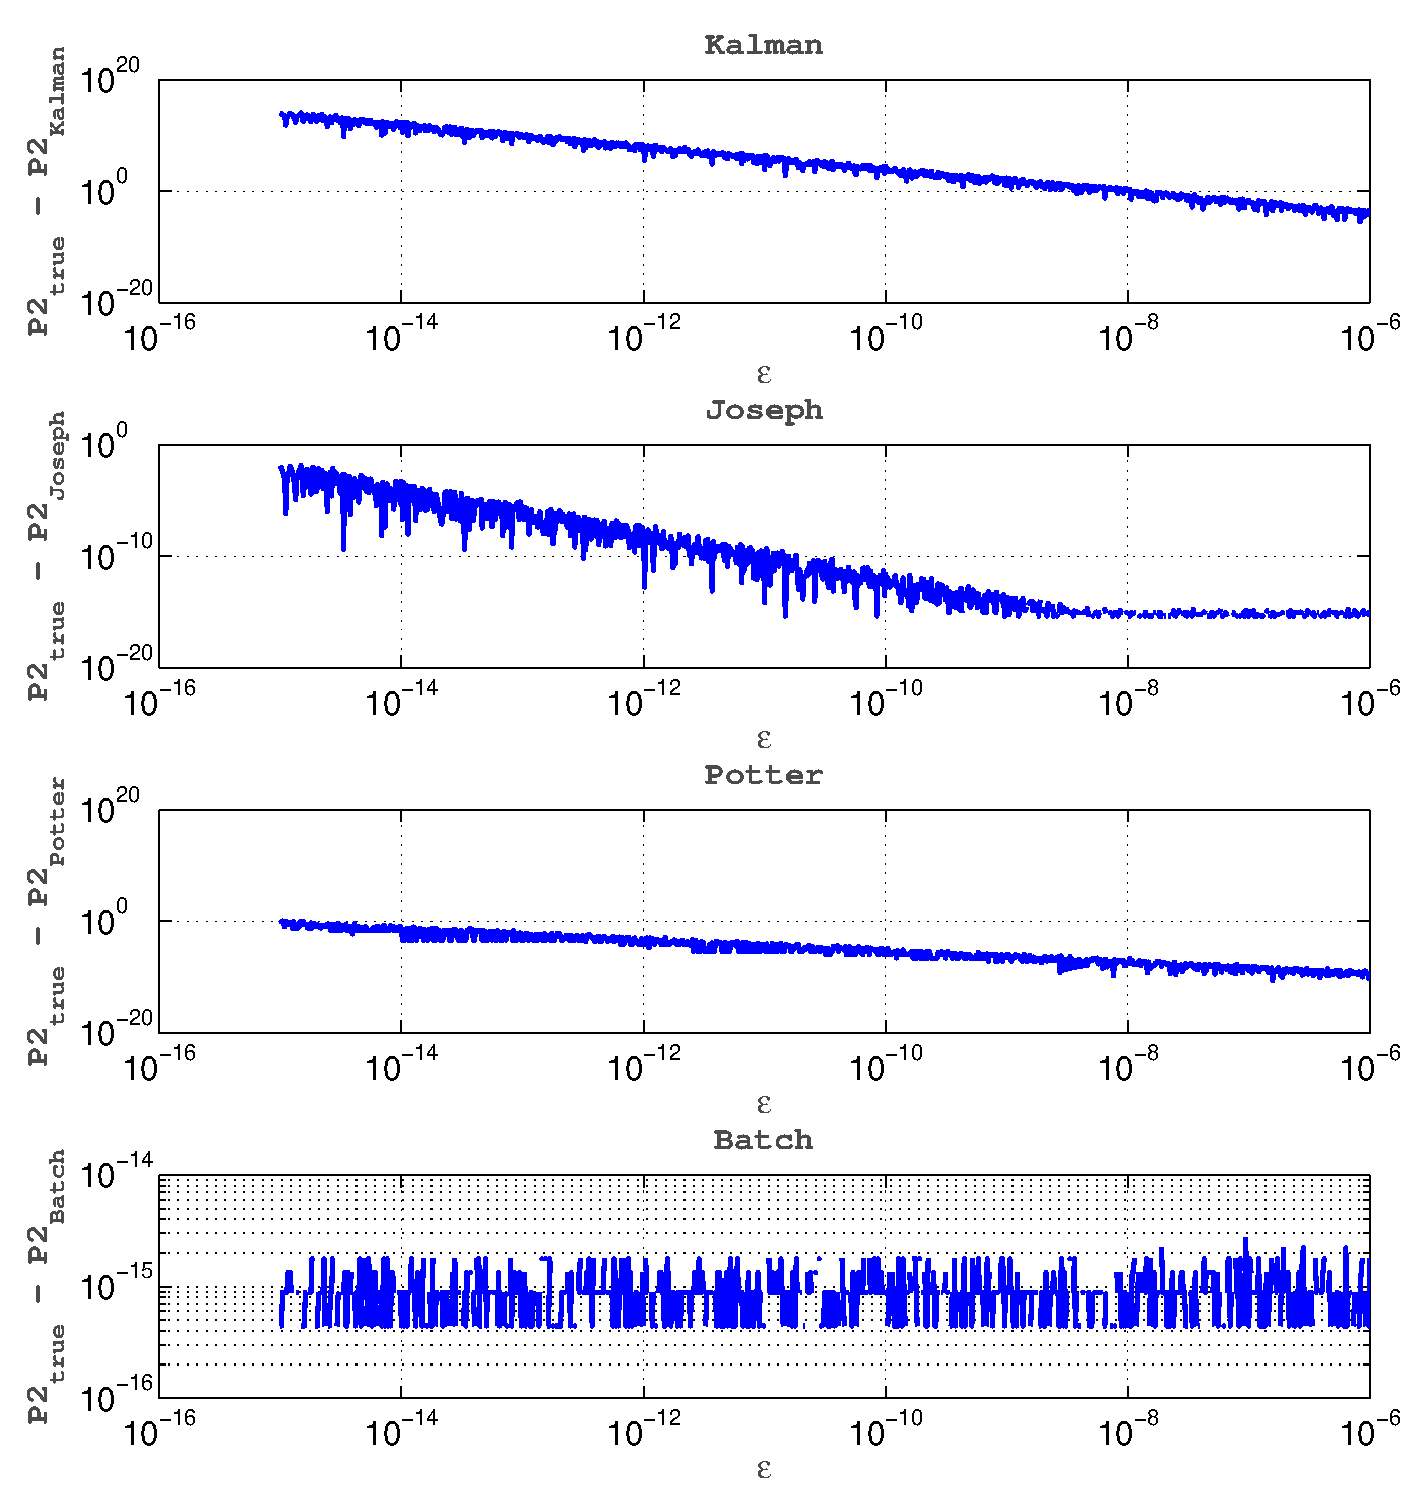
\includegraphics [width=4in]{HW8main_02.eps}

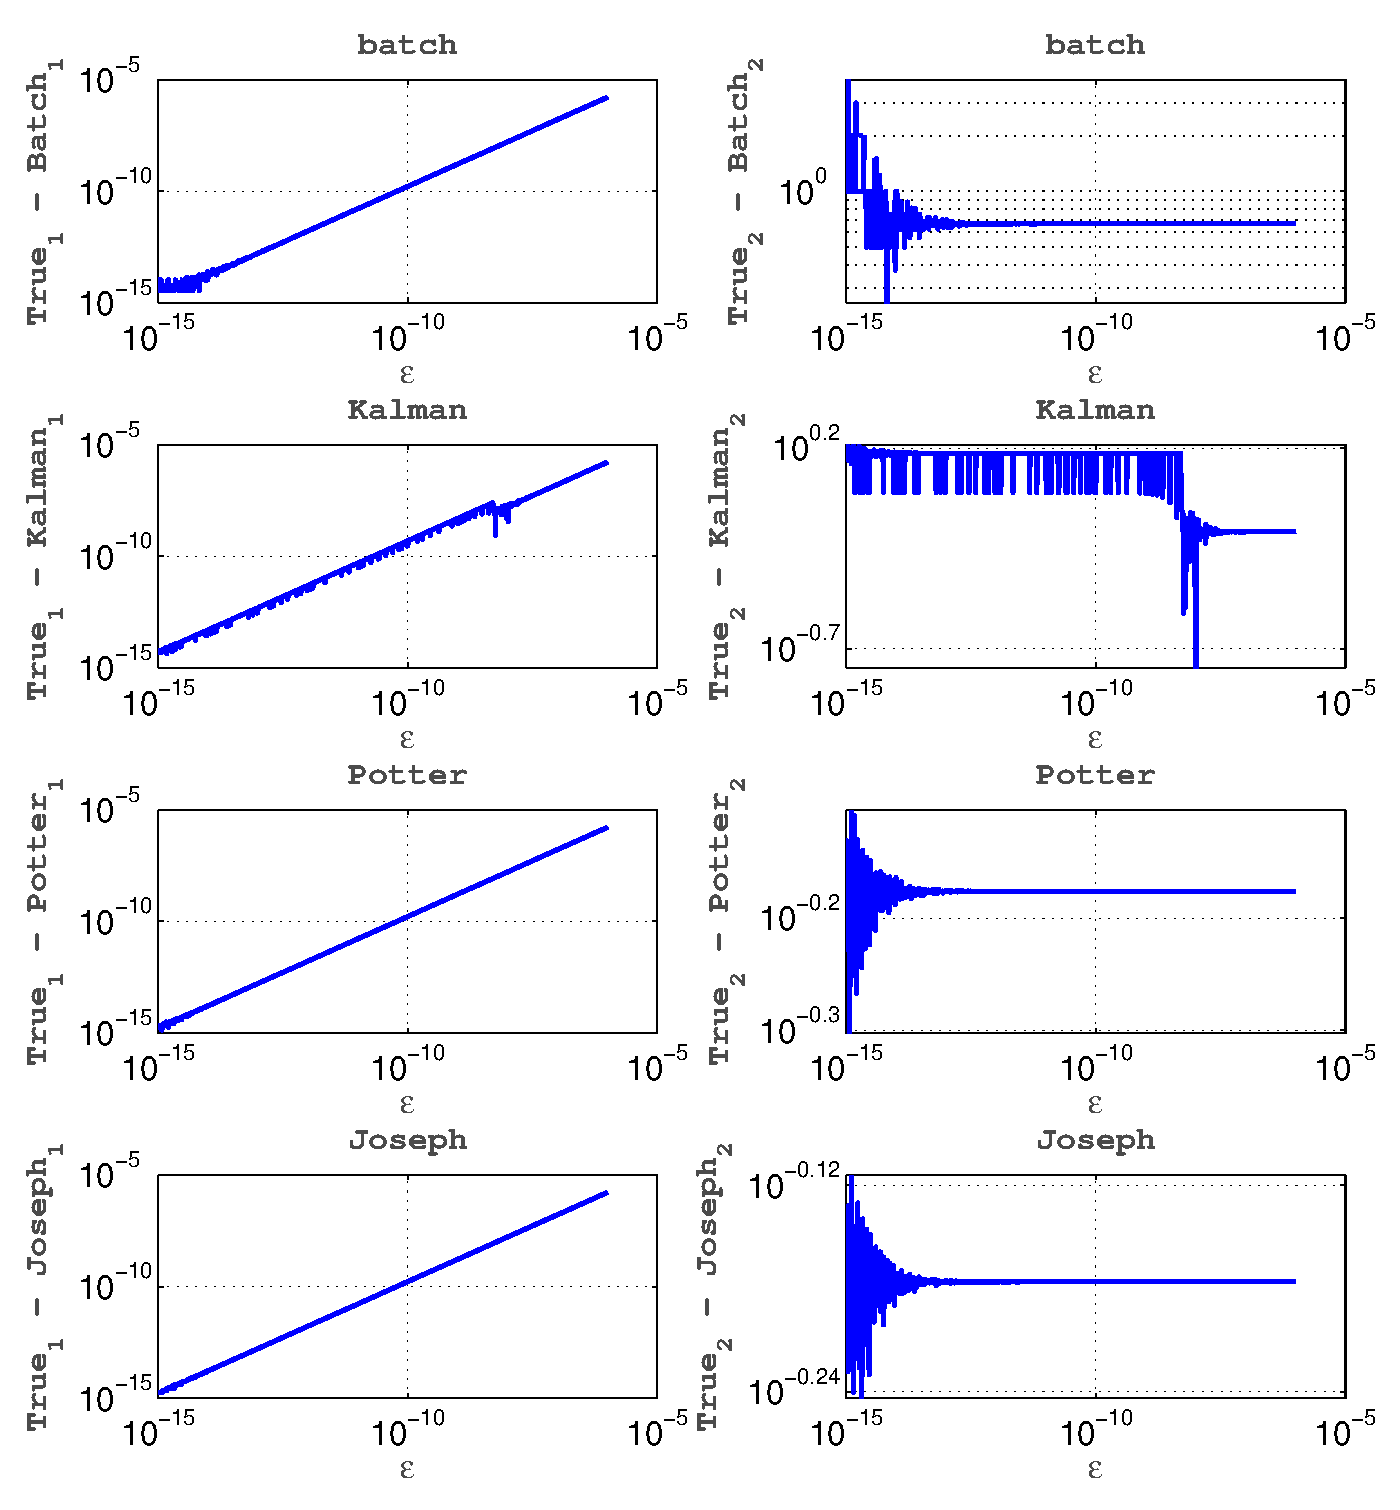
\includegraphics [width=4in]{HW8main_03.eps}



\end{document}
    
